%!TEX root=../../autopilot.tex
\section{Stimuli}
\label{sec:stim}

\begin{marginfigure}[0.45cm]
\begin{pythoncode*}{
label= \texttt{An Autopilot Tone},
frame=lines,
linenos=false}

my_tone = sounds.Tone(
    frequency = 500,
    duration  = 200)
my_tone.play()
\end{pythoncode*}
\vspace{-18pt}
\begin{matlabcode*}{
label=\texttt{A \href{https://github.com/sanworks/Bpod_Gen2/blob/master/Examples/Protocols/AnalogSound2AFC/AnalogSound2AFC.m}{Bpod Tone}},
frame=lines,
linenos=false}
tone = GenerateSineWave(...
samplingrate, freq, dur);

% load to audio server
server = BPodAudioPlayer;
server.loadSound(1,tone);

% buffer sound after poke
sma = AddState(sma, ...,
'OutputActions', 
{'AudioPlayer1', '*'});
% play sound by number
sma = AddState(sma, ...,
'OutputActions',
{'AudioPlayer1', 1});
\end{matlabcode*}
\caption{Autopilot stimuli are parametrically defined and inherit all the playback logic that makes them easy to integrate in tasks}
\label{fig:tone}
\end{marginfigure}

A hardware object would control a speaker, whereas stimulus objects are the individual sounds that the speaker would play. Like tasks and hardware, Autopilot makes stimulus generation portable between users, and is released with a family of common sounds like tones, noises, and sounds from files. The logic of sound presentation is contained in an inherited metaclass, so to program a new stimulus a user only needs to describe how to generate it from its parameters (Figure \ref{fig:tone}).  Sound stimuli are better developed than visual stimuli in the current version of Autopilot, but we present a proof-of-concept visual experiment (Section \ref{sec:gonogo}) using \href{https://www.psychopy.org/}{psychopy}\citep{peircePsychoPy2ExperimentsBehavior2019}.

Autopilot controls the realtime audio server \href{http://jackaudio.org/}{jack} from an independent Python process that dumps samples directly into jack's buffer (Figure \ref{fig:soundpath}), giving it the lowest trigger-to-playback latency of any of the systems we have tested or found benchmarks for (Section \ref{sec:latency}). Sounds can be buffered in system memory or synthesized on demand, and the only limit on the number of stimuli that can be simultaneously buffered is the Pi's generous 4GB of memory. Because the realtime server is independent from the logic of sound synthesis and storage, stimuli can be controlled independently from different threads without interrupting audio or dropping frames.

We use the \href{https://www.hifiberry.com/shop/boards/hifiberry-amp2/}{Hifiberry Amp 2}, a combined sound card and amplifier, which is capable of 192kHz/24Bit audio playback. Jack can output to any sound hardware, however, including the builtin audio of the Raspberry Pi if fidelity isn't important. There are no external video cards for the Raspberry Pi, but its embedded video card is capable of presenting video and visual stimuli (Section \ref{sec:gonogo}) especially if the other computationally demanding parts of the task are distributed to other Raspberry Pis (Section \ref{sec:topology}).

\begin{marginfigure}[0cm]
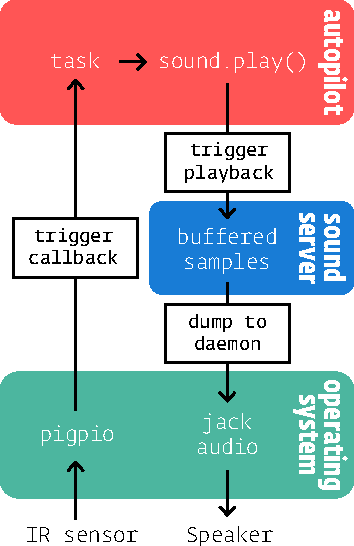
\includegraphics[]{figures/side_19_soundpath.pdf}
\caption{Our sound server keeps audio samples buffered until a \texttt{.play()} method is called, and then dumps them directly into the jack audio daemon.}
\label{fig:soundpath}
\end{marginfigure}

\subsection{Stimulus and Reward Managers}
\label{sec:managers}

In many tasks, the structure of the stimulus presentation is as important as the structure of the task. Stimulus structure can become complicated quickly---in addition to whatever order is necessitated by the task design, it is common to also include shaping routines like bias correction in the presentation logic. Different types of stimuli also require different degrees of coordination: unitary stimuli that are presented once per trial can be handled independently without fear of them overlapping  or interrupting one another, but continuous stimuli that change in response to task performance need to be mutually coordinated. 

We separate stimulus presentation logic from task structure by using stimulus managers. Stimulus managers have different 'base' presentation types---eg. random presentation, blocked presentation, etc.---and a set of configurable transformations like bias correction that can be chained together. The stimulus manager can yield prebuffered stimulus objects, synthesize new stimuli according to some task-related rule, and manage a continuous stimulus stream. 

Reward managers behave similarly\sidenote{Reward managers are not yet implemented as independent classes in the current version (0.2) of Autopilot, but are a planned feature of Autopilot v0.3. Different modes of reward delivery are currently implemented by the \href{http://docs.auto-pi-lot.com/autopilot.core.hardware.html\#autopilot.core.hardware.Solenoid}{\texttt{Solenoid} class}.}. Reward managers can implement different calibration schemes---eg. for gravity-fed water delivery, reward can be configured to be delivered for a constant time, constant volume, or use the animal's mass and performance to adaptively deliver a total volume over a period of time.